%
% $RCSfile: short_and_long_term_memory.tex,v $
%
% Copyright (C) 2002-2008. Christian Heller.
%
% Permission is granted to copy, distribute and/or modify this document
% under the terms of the GNU Free Documentation License, Version 1.1 or
% any later version published by the Free Software Foundation; with no
% Invariant Sections, with no Front-Cover Texts and with no Back-Cover
% Texts. A copy of the license is included in the section entitled
% "GNU Free Documentation License".
%
% http://www.cybop.net
% - Cybernetics Oriented Programming -
%
% http://www.resmedicinae.org
% - Information in Medicine -
%
% Version: $Revision: 1.1 $ $Date: 2008-08-19 20:41:08 $ $Author: christian $
% Authors: Christian Heller <christian.heller@tuxtax.de>
%

\subsection{Short- and Long-Term Memory}
\label{short_and_long_term_memory_heading}
\index{Short-Term Memory}
\index{STM}
\index{Long-Term Memory}
\index{LTM}
\index{Sensory Memory}
\index{Psychology}
\index{Persistent Storage}
\index{Transient Storage}

It was previously worked out that there are brain regions mainly storing and
applying knowledge and others controlling the input/ output (i/o) and
manipulation of that knowledge. \emph{Learning}, \emph{Storage} and
\emph{Recall} of knowledge are main tasks of the human brain, which are studied
by the science of \emph{Psychology}.

Besides the \emph{persistent} storage in \emph{Long Term Memory} (LTM), the brain
is capable of storing \emph{transient} information in \emph{Short Term Memory}
(STM), the latter also being called \emph{primary} or \emph{active} memory
\cite{wikipedia}. An additional \emph{Sensory Memory} stores information arriving
directly from the corresponding organs. Figure \ref{memory_figure} tries to
classify \emph{some} types of memory, as described by psychology. It is not
more than a \emph{trial} because psychology itself is not sure about memory
classification and several theories exist.

\begin{figure}[ht]
    \begin{center}
        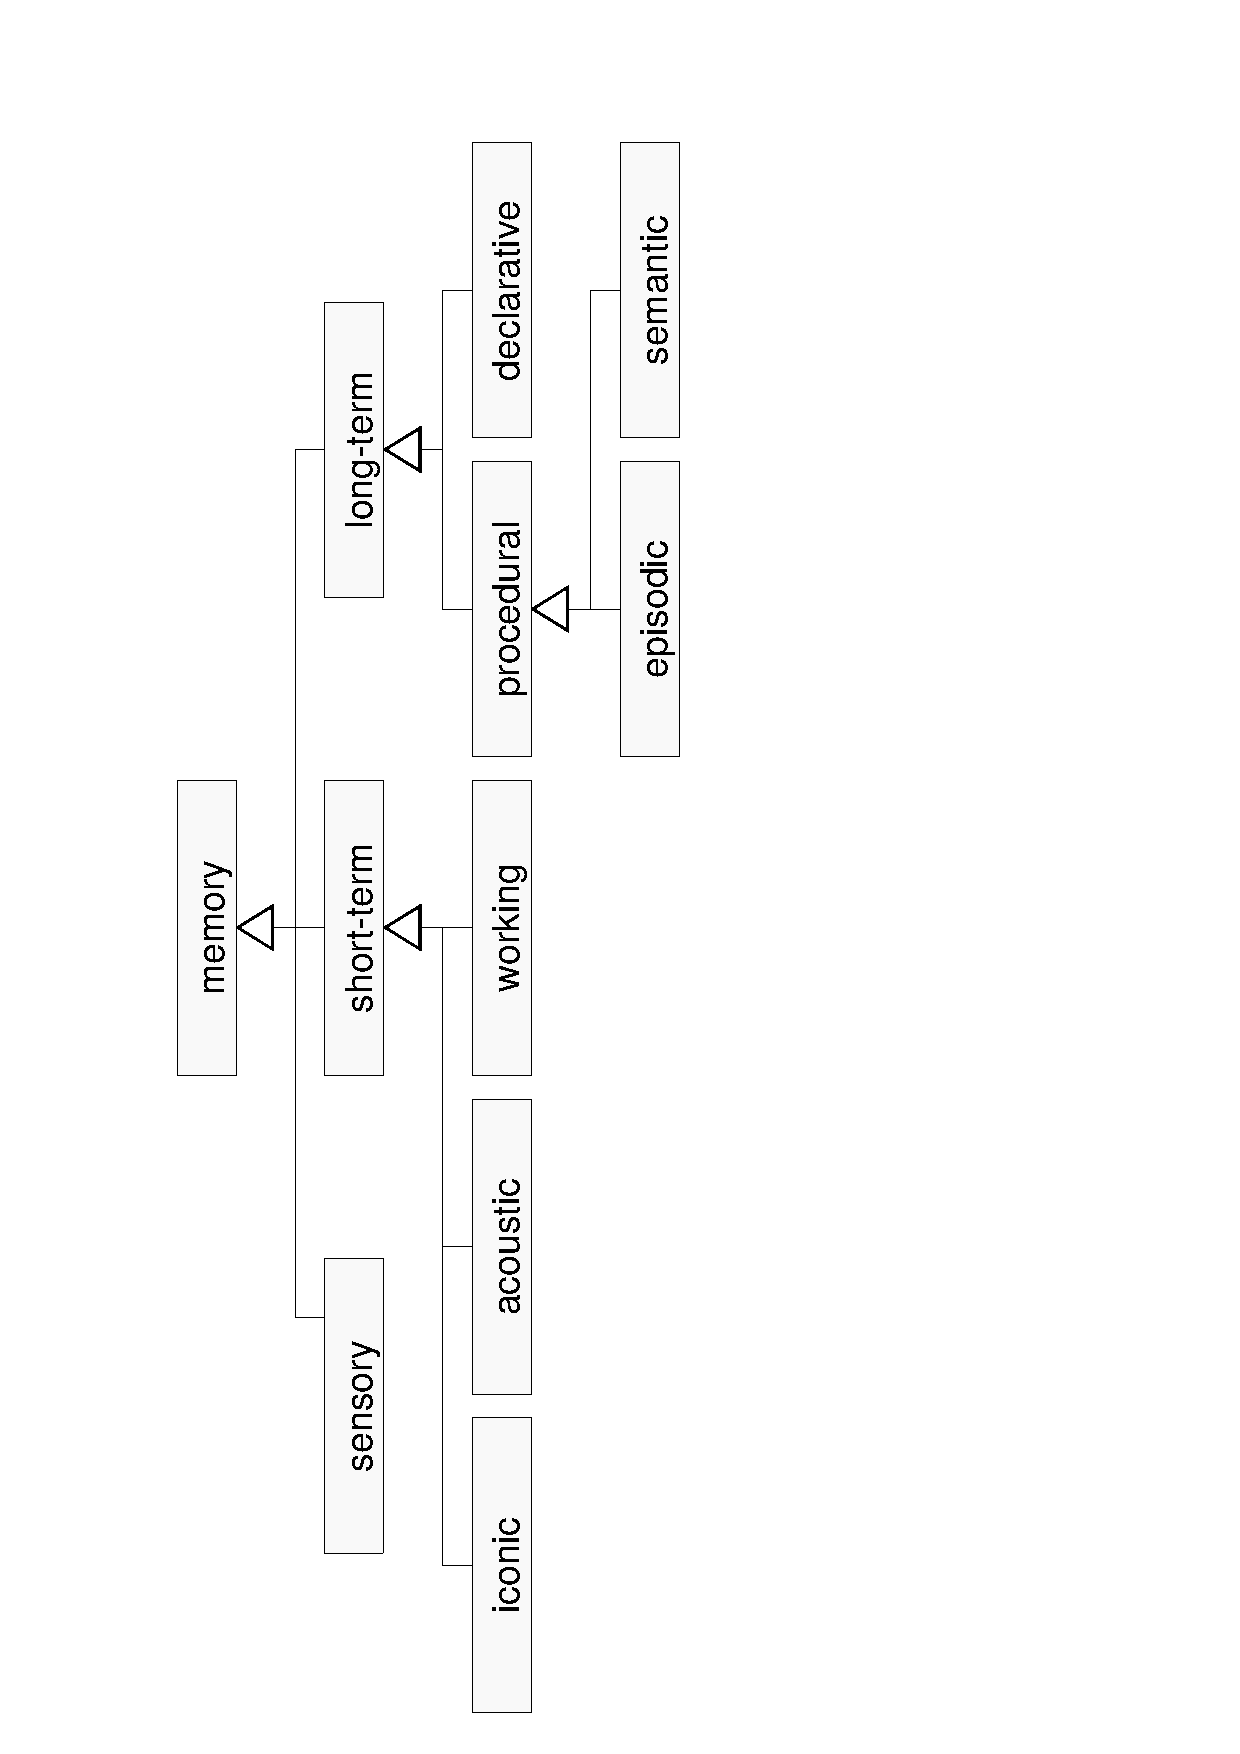
\includegraphics[scale=0.3,angle=-90]{graphic/memory.pdf}
        \caption{Types of Memory \cite{lai, eet}}
        \label{memory_figure}
    \end{center}
\end{figure}

The \emph{Encyclopedia of Educational Technology} (EET) \cite{eet} writes:

\begin{quote}
    The sensory information store has unlimited capacity, and reacts to both
    visual and auditory information. However, the duration of information in
    sensory memory is extremely brief, perhaps only 300 miliseconds, and is
    subject to rapid decay.

    STM, in general, is characterized by a limited capacity of up to seven
    pieces of independent information, and in the brief duration of these items
    in STM, usually anywhere from three to 20 seconds. Additionally, decay
    appears to be the primary mechanism of memory loss in STM.

    LTM efficiently stores our knowledge about the world. It is important to
    contrast LTM with other types of memory and understand how it is
    structured. The knowledge we store in LTM affects our perceptions of the
    world, and influences what information in the environment we attend to. LTM
    provides the framework to which we attach new knowledge, and its properties
    have important implications for instructional design.
\end{quote}

In the words of the Free Wikipedia Encyclopedia \cite{wikipedia}, Information
held in STM may be: \textit{recently processed sensory input; items recently
retrieved from LTM; or the result of recent mental processing.} When doing
mathematical calculations, for example, intermediary results stored in STM are
available for only a short time and forgotten soon after.

The \emph{declarative} LTM is conscious memory, a \emph{film} of past contents
\cite{fernandez}. The \emph{procedural} -- or \emph{non-declarative} -- LTM is
unconscious memory which enables humans to carry out a task (like riding a
bicycle), without having to consciously control it. In other words, procedures
stored in non-declarative LTM are available- and may run as background program.

What effects do these reflections have on the design of software systems? The
storage and dynamic processing of static knowledge may firstly rely on at least
two different kinds of memory, one for \emph{persistent-} and another one for
\emph{transient} storage of knowledge; secondly, they may rely not only on one
main process controlling the system, but (as equivalent to procedural LTM)
employ a number of background processes solving special tasks.
